\chapter{Исследовательский раздел}
В данном разделе проводится исследование эффективности разработанного метода распознавания спортивных действий человека. Проводится исследование метрик модели в зависимости от разметки данных. Описываются исследования характеристик разработанного метода, а именно исследование результатов распознавания модели в зависимости от контрастности видео и исследование результатов распознавания модели в зависимости от качества видео.

\section{Исследование метрик модели в зависимости от разметки данных}

В качестве метрик оценки классификации были выбраны общая точность предсказания модели (accuracy), точность (precision) и полнота (recall).
Величина метрик вычислялась, как среднее значение метрик на каждой итерации алгоритма кросс-валидации.

Перекрестная проверка (кросс-валидация) -- это процедура повторной выборки, используемая для оценки моделей машинного обучения на ограниченной выборке данных.

Процедура имеет один параметр, называемый k, который относится к числу групп, на которые должна быть разделена данная выборка данных. Таким образом, процедура часто называется  k-fold кросс-валидацией (перекрестной проверкой).

 Так как основной набор данных содержал неодинаковое количество видео в каждом классе, использовался метод стратификации, а именно при разбиении на тестовый и тренировочный набор на каждой итерации алгоритма, данные распределены так, что каждый набор содержит примерно такое же соотношение классов, как и всё исходное множество. Каждый кадр видео после предсказания относится к одной из ситуаций, которые более подробно описаны в разделе \ref{test}:


\begin{itemize}
	\item[---]  TP -- истинно-положительное решение;
	\item[---] TN -- истинно-отрицательное решение;
	\item[---]  FP -- ложно-положительное решение;
	\item[---]  FN -- ложно-отрицательное решение.

\end{itemize}

На каждой итерации цикла кросс-валидации на основе вычисленных выше описанных переменных можно рассчитать величины метрик.

Если рассмотреть долю правильно предсказанных положительных объектов среди всех объектов, предсказанных положительным классом, то можно получить метрику, которая называется точностью (precision). Точность рассчитывается по следующей формуле:

\begin{equation}
	Precision =  \frac{TP}{TP + FP}.
\end{equation}

Доля правильно найденных положительных объектов среди всех объектов положительного класса, называется полнотой (recall). Полнота рассчитывается по следующей формуле:

\begin{equation}
	Recall =  \frac{TP}{TP + FN} .
\end{equation}

Accuracy -- это показатель, который описывает общую точность предсказания модели по всем классам. Это особенно полезно, когда каждый класс одинаково важен. Он рассчитывается как отношение количества правильных прогнозов к их общему количеству:

\begin{equation}
	Accuracy =  \frac{TP + TN}{TP + FN + TN + FT}.
\end{equation}

Метрики рассчитывались для двух моделей, обученных на данных с разной разметкой. В первом случае при формировании дескрипторов метка назначалась на каждое видео, в другом на дескриптор каждого кадра, в этом случае предсказанное действие выбиралось как чаще всего встречающиеся предсказанная метка среди кадров. Результаты исследования представлены на рисунке 4.1.

\begin{figure}[h]
	\begin{center}
		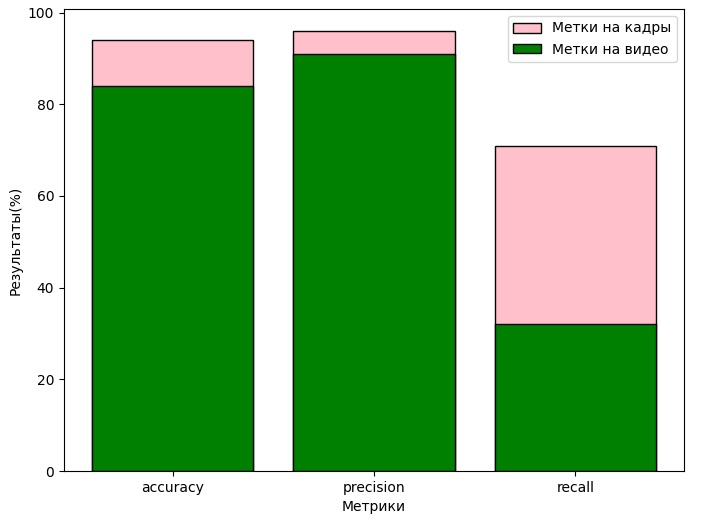
\includegraphics[ scale=0.6]{./img/exp1.jpg}
		\caption{Зависимость метрик модели от разметки данных}  
		\label{fig:xray1}
	\end{center}
\end{figure}

По столбчатым диаграммам  можно заметить, что при назначении метки на каждый кадр метрика полнота выросла в два раза. Это показывает, что при назначении метки на каждое видео меньше половины объектов положительного класса были не распознаны моделью, это является плохим показателем, при разметки на каждый кадр метрика растет до 76\%, что уже является оптимальным показателем. Остальные метрики при разметки на каждый кадр также выше, но не значительно.

\section{Исследование результатов распознавания модели в зависимости от контрастности видео}

Для проведения этого исследования тестовая выборка каждого класса на основе экспертной оценки была разделена на видео высокой контрастности и низкой. Далее для каждого видео предсказывался вид действия и считалось количество верно распознанных действий для каждого класса. На основе рассчитанного количества верно распознанных действий рассчитывался процент верного распознания каждого класса действий в зависимости от контрастности, как отношение верно распознанных к общему количеству видео в соответствующей выборке. Тестовые выборки, разделенные по контрастности содержали видео только высокого качества. На рисунке 4.2 представлены результаты проведенного исследования.
\clearpage
\begin{figure}[h]
	\begin{center}
		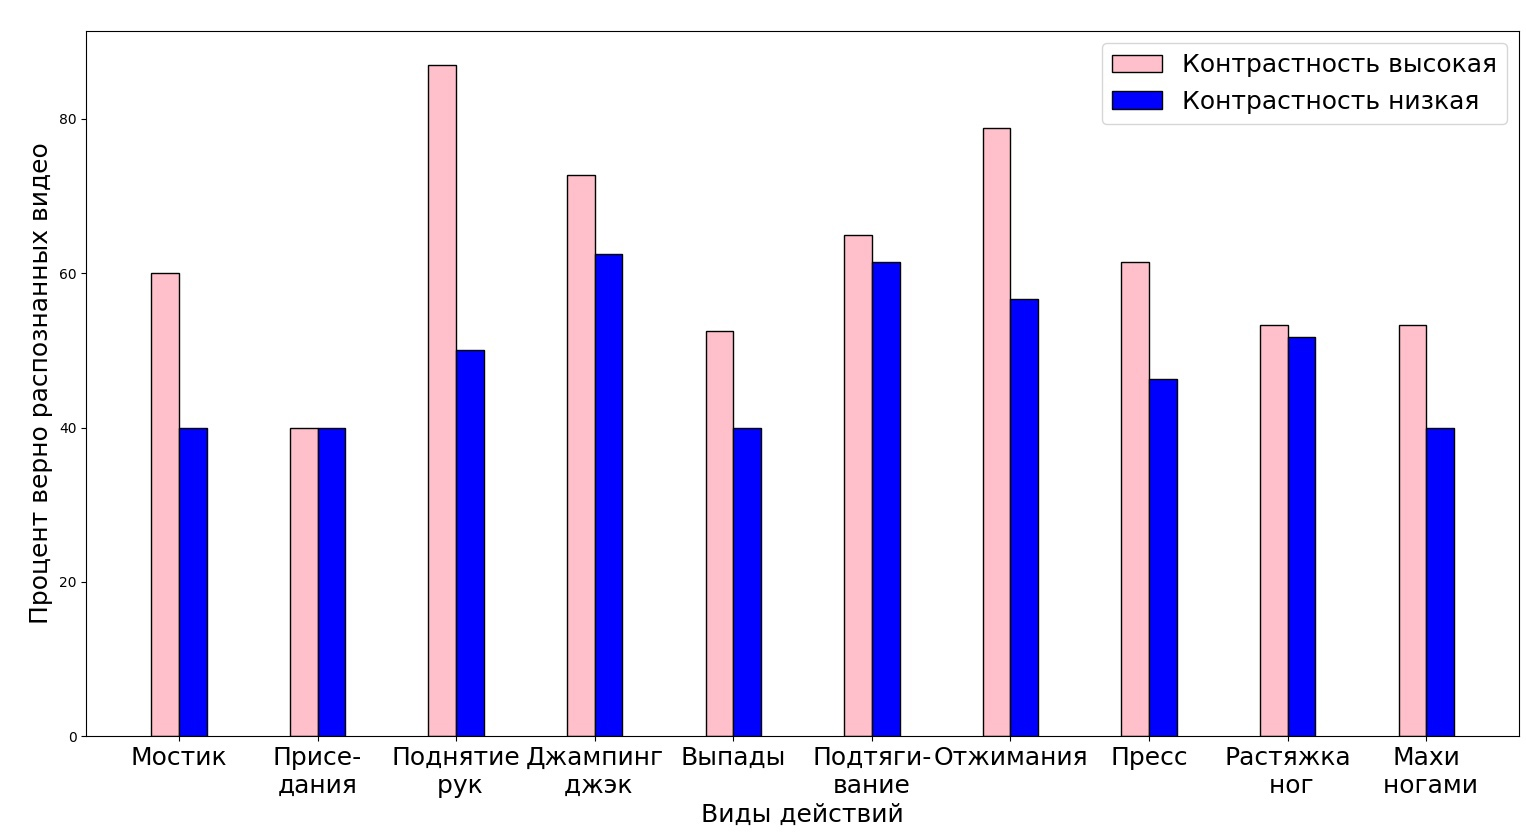
\includegraphics[ scale=0.32]{./img/exp3.jpg}
		\caption{Зависимость результатов распознавания от контрастности видео}  
		\label{fig:xray1}
	\end{center}
\end{figure}

В результате можно сделать вывод о том, что видео высокой контрастности модель распознает с меньшим количеством ошибок засчет того, что при резких переходах цвета на кадре градиенты интенсивностей больше.

\section{Исследование результатов распознавания модели в зависимости от качества видео}

Для проведения этого исследования тестовая выборка каждого класса была разделена на видео высокого и низкого качества. В связи с ограниченностью набора данных за высокое качество были приняты видео размером больше 256х256 пикселей, а за низкого размером меньше 256х256 пикселей. Выборка состояла из видео высокой контрастности и проводилось только на некоторых видах действий в связи с отсутствием достаточного количества видео низкого качества в исходном наборе данных. Далее для каждого видео предсказывался вид действия и считалось количество верно распознанных действий для каждого класса. На основе рассчитанного количества верно распознанных действий рассчитывался процент верного распознания каждого класса действий в зависимости от качества, как отношение верно распознанных к общему количеству видео в соответствующей выборке. На рисунке 4.3 представлены результаты проведенного исследования.

\begin{figure}[h]
	\begin{center}
		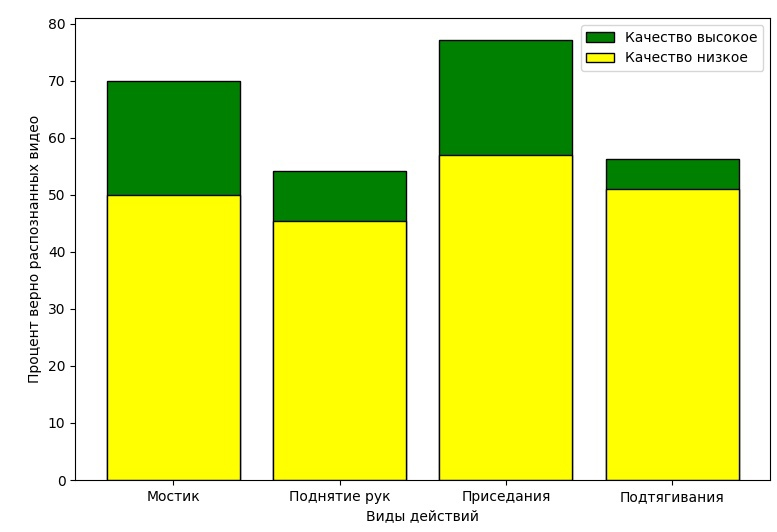
\includegraphics[ scale=0.6]{./img/exp2.jpg}
		\caption{Зависимость результатов распознавания от качества видео}  
		\label{fig:xray1}
	\end{center}
\end{figure}

\section{Выводы}
В результате проведенных исследований можно сделать вывод о том, что модель имеет более высокие показатели метрик при назначение метки на дескриптор каждого кадра, нежели при назначение на дескриптор видео.

Так же исследования показали, что на видео высокого качества на выборке, состоящей из контрастных видео, модель ошибается меньшее количество раз, нежели на видео низкого качества.

Модель чаще ошибается при распознавании видео с низкой контрастностью, нежели с высокой на выборке из видео высокого качества.

